% Build from the repository root: make -C presentation
% Presentation order: running example -> reading diagrams -> composition -> quantales
% -> inherited GPA -> the GLP extension -> epigraph completeness -> scope.
% Exactly 27 frames; no overlays or hidden appendix slides.
\documentclass[aspectratio=169,12pt]{beamer}
\usepackage[english]{babel}
\usepackage{amsmath,amssymb}
\usepackage{tikz}
\usetikzlibrary{shapes,arrows,arrows.meta,intersections,bending,calc,positioning,fit,backgrounds}
\input{../material/generator.tikzstyles}
% Every pic occupies the uniform frame x in [-0.5, 0.5], y in [-0.5, 0.5].
% Tips live on the left/right edges as (-in-k) / (-out-k), top-first,
% evenly spaced in [-0.5, 0.5]: for n tips, y_k = 0.5 - k/(n-1) (n >= 2),
% or y_0 = 0 when n = 1. Codegen relies on this convention to align tips
% across composition without needing tip data in JSON.
%
% Coloured node glyphs (whitedot / boxnode_*) are drawn *after* the wires so
% the fill covers any wire segment passing through the node interior.
\tikzset{
  val/.store in = \argval,
  multiplication/.pic = {
    \coordinate (-in-0)  at (-0.5, 0.5);
    \coordinate (-in-1)  at (-0.5,-0.5);
    \coordinate (-out-0) at ( 0.5, 0);
    \draw (-in-0) to[bend left=30]  (0,0);
    \draw (-in-1) to[bend right=30] (0,0);
    \draw (0,0)   to (-out-0);
    \node[whitedot] (-node) at (0,0) {};
  },
  comultiplication/.pic = {
    \coordinate (-out-0)  at (0.5, 0.5);
    \coordinate (-out-1)  at (0.5,-0.5);
    \coordinate (-in-0) at ( -0.5, 0);
    \draw (-out-0) to[bend right=30]  (0,0);
    \draw (-out-1) to[bend left=30] (0,0);
    \draw (0,0)   to (-in-0);
    \node[whitedot] (-node) at (0,0) {};
  },
  zero/.pic = {
    \coordinate (-out-0) at (0.5, 0);
    \draw (0,0) to (-out-0);
    \node[whitedot] (-node) at (0,0) {};
  },
  cozero/.pic = {
    \coordinate (-in-0) at (-0.5, 0);
    \draw (-in-0) to (0,0);
    \node[whitedot] (-node) at (0,0) {};
  },
  copy/.pic = {
    \coordinate (-out-0)  at (0.5, 0.5);
    \coordinate (-out-1)  at (0.5,-0.5);
    \coordinate (-in-0) at (-0.5, 0);
    \draw (-out-0) to[bend right=20]  (0,0);
    \draw (-out-1) to[bend left=20] (0,0);
    \draw (0,0)   to (-in-0);
    \node[blackdot] (-node) at (0,0) {};
  },
  cocopy/.pic = {
    \coordinate (-in-0)  at (-0.5, 0.5);
    \coordinate (-in-1)  at (-0.5,-0.5);
    \coordinate (-out-0) at ( 0.5, 0);
    \draw (-in-0) to[bend left=20]  (0,0);
    \draw (-in-1) to[bend right=20] (0,0);
    \draw (0,0)   to (-out-0);
    \node[blackdot] (-node) at (0,0) {};
  },
  discard/.pic = {
    \coordinate (-in-0) at (-0.5, 0);
    \draw (-in-0) to (0,0);
    \node[blackdot] (-node) at (0,0) {};
  },
  codiscard/.pic = {
    \coordinate (-out-0) at (0.5, 0);
    \draw (0,0) to (-out-0);
    \node[blackdot] (-node) at (0,0) {};
  },
  scalar/.pic = {
    \coordinate (-in-0)  at (-0.5, 0);
    \coordinate (-out-0) at ( 0.5, 0);
    \draw (-in-0) to (0,0);
    \draw (0,0)   to (-out-0);
    \node[boxnode_right] (-node) at (0,0) {$\argval$};
  },
  coscalar/.pic = {
    \coordinate (-in-0)  at (-0.5, 0);
    \coordinate (-out-0) at ( 0.5, 0);
    \draw (-in-0) to (0,0);
    \draw (0,0)   to (-out-0);
    \node[boxnode_left] (-node) at (0,0) {$\argval$};
  },
  matrix/.pic = {
    \coordinate (-in-0)  at (-1.0, 0);
    \coordinate (-out-0) at ( 1.0, 0);
    \draw (-in-0) to (0,0);
    \draw (0,0)   to (-out-0);
    \node[matrixnode_left] (-node) at (0,0) {$\argval$};
  },
  comatrix/.pic = {
    \coordinate (-in-0)  at (-1.0, 0);
    \coordinate (-out-0) at ( 1.0, 0);
    \draw (-in-0) to (0,0);
    \draw (0,0)   to (-out-0);
    \node[matrixnode_right] (-node) at (0,0) {$\argval$};
  },
  2dmatrix/.pic = {
    \coordinate (-in-0)  at (-1.0, 0.3);
    \coordinate (-in-1)  at (-1.0, -0.3);
    \coordinate (-out-0) at ( 1.0, 0);
    \draw (-in-0) to (0,0.3);
    \draw (-in-1) to (0,-0.3);
    \draw (0,0)   to (-out-0);
    \node[matrixnode_left] (-node) at (0,0) {$\argval$};
  },
  2dcomatrix/.pic = {
    \coordinate (-in-0)  at (-1.0, 0);
    \coordinate (-out-0) at ( 1.0, -0.5);
    \coordinate (-out-1) at ( 1.0, 0.5);
    \draw (-in-0) to (0,0);
    \draw (0,0)   to (-out-0);
    \node[matrixnode_right] (-node) at (0,0) {$\argval$};
  },
  relation/.pic = {
    \coordinate (-in-0)  at (-1.0, 0);
    \coordinate (-out-0) at ( 1.0, 0);
    \draw (-in-0) to (0,0);
    \draw (0,0)   to (-out-0);
    \node[relationnode_right] (-node) at (0,0) {$\argval$};
  },
  corelation/.pic = {
    \coordinate (-in-0)  at (-1.0, 0);
    \coordinate (-out-0) at ( 1.0, 0);
    \draw (-in-0) to (0,0);
    \draw (0,0)   to (-out-0);
    \node[relationnode_left] (-node) at (0,0) {$\argval$};
  },
  2drelation/.pic = {
    \coordinate (-in-0)  at (-1.0, 0.3);
    \coordinate (-in-1)  at (-1.0, -0.3);
    \coordinate (-out-0) at ( 1.0, 0);
    \draw (-in-0) to (0,0.3);
    \draw (-in-1) to (0,-0.3);
    \draw (0,0)   to (-out-0);
    \node[relationnode_right] (-node) at (0,0) {$\argval$};
  },
  2dcorelation/.pic = {
    \coordinate (-in-0)  at (-1.0, 0);
    \coordinate (-out-0) at ( 1.0, -0.5);
    \coordinate (-out-1) at ( 1.0, 0.5);
    \draw (-in-0) to (0,0);
    \draw (0,0)   to (-out-0);
    \node[relationnode_left] (-node) at (0,0) {$\argval$};
  },
  affine/.pic = {
    \coordinate (-out-0) at (0.5, 0);
    \draw (0,0) to (-out-0);
    \node (-node) at (0,0) {$|$};
  },
  coaffine/.pic = {
    \coordinate (-out-0) at (-0.5, 0);
    \draw (0,0) to (-out-0);
    \node (-node) at (0,0) {$|$};
  },
  ge/.pic = {
    \coordinate (-in-0)  at (-0.5, 0);
    \coordinate (-out-0) at ( 0.5, 0);
    \draw (-in-0) to (0,0);
    \draw (0,0)   to (-out-0);
    \node[boxnode_right] (-node) at (0,0) {$\ge$};
  },
  coge/.pic = {
    \coordinate (-in-0)  at (-0.5, 0);
    \coordinate (-out-0) at ( 0.5, 0);
    \draw (-in-0) to (0,0);
    \draw (0,0)   to (-out-0);
    \node[boxnode_left] (-node) at (0,0) {$\le$};
  },
  linear/.pic = {
    \coordinate (-out-0) at (0.5, 0);
    \draw (0,0) to (-out-0);
    \node[leftseminode] (-node) at (0,0) {};
  },
  relu/.pic = {
    \coordinate (-in-0)  at (-0.5, 0);
    \coordinate (-out-0) at (0.5, 0);
    \draw (-in-0) to (0,0);
    \draw (0,0)   to (-out-0);
    \node[draw, fill=white] (-node) at (0,0) {ReLU};
  },
  antipode/.pic = {
    \coordinate (-in-0) at (-0.5, 0);
    \coordinate (-out-0) at (0.5, 0);
    \draw (-in-0) to (0,0);
    \draw (0,0) to (-out-0);
    \node[draw, fill=black] (-node) at (0,0) {};
  },
  diagram/.pic = {
    \coordinate (-in-0)  at (-0.5, 0);
    \coordinate (-out-0) at ( 0.5, 0);
    \draw (-in-0) to (0,0);
    \draw (0,0)   to (-out-0);
    \node[diagram] (-node) at (0,0) {$\argval$};
  }
}

% Classic Beamer theme (Madrid) and shared diagram helpers.
\usetheme{Madrid}
\usecolortheme{default}
\usefonttheme{default}
\setbeamertemplate{navigation symbols}{}

% Emphasis in the structure colour instead of an ad-hoc palette.
\newcommand{\hl}[1]{{\color{structure}\bfseries #1}}
\newcommand{\credit}[1]{\par\vspace{1mm}{\tiny\color{black!55} #1\par}}
\newcommand{\tagline}[1]{\begin{block}{Takeaway}\bgroup\normalfont\small #1\egroup\end{block}}

\tikzset{
  process/.style={draw=black,thick,rounded corners=1.5mm,fill=white,
    minimum width=1cm,minimum height=.7cm,inner sep=3mm},
  stage/.style={draw=black,thick,rounded corners=1.5mm,fill=white,
    minimum width=2.2cm,minimum height=1.2cm,align=center,inner sep=3mm,font=\small},
  proofbox/.style={draw=black,thick,rounded corners=1.5mm,fill=white,
    minimum height=.85cm,align=center,inner sep=2.5mm,font=\small},
  wire/.style={draw=black,thick},
  axpic/.style={baseline=(current bounding box.center),line cap=round}
}


 \newcommand{\inlinegen}[1]{
    \begin{tikzpicture}
        \pic {#1};
    \end{tikzpicture}
}
\newcommand{\sem}[1]{[\![#1]\!]}
\newcommand{\ind}[1]{\mathcal I_{#1}}
\newcommand{\GPA}{\mathbf{GPA}}
\newcommand{\GLP}{\mathbf{GLP}}
\newcommand{\LPRel}{\mathbf{LPRel}}
\newcommand{\PolyRel}{\mathbf{PolyRel}}
\newcommand{\epi}{\operatorname{epi}}
\newcommand{\diagrow}[3]{#1 & \begin{tikzpicture}[baseline=(current bounding box.center)]#2\end{tikzpicture} & $=$ & \begin{tikzpicture}[baseline=(current bounding box.center)]#3\end{tikzpicture}\\[2mm]}
\newcommand{\costpic}{\begin{tikzpicture}[baseline=(current bounding box.center),scale=1.5]\pic (l) at (0,0) {linear};\node[above] at (0,.32) {$\ell$};\node[right] at (.55,0) {$x$};\end{tikzpicture}}

% Running example (frames 2, 3, 17): min x1 + 2 x2  s.t.  0 <= x1 <= 1, x2 >= 0,
% x1 + x2 >= d.  Value function v(d) = max{0, d, 2d - 1}.
\newcommand{\valueplot}{%
\begin{tikzpicture}[scale=1.05,thin]
\draw[->] (0,0) -- node[right,font=\small]{} (3.95,0);
\draw[->] (0,0) -- node[left,font=\small]{$v(d)$} (0,4.45);
\draw (1,0) -- (1,0.08) node[below,font=\small]{$1$};
\draw[very thick] (-0.,0) -- (1,1) -- (2.45,3.9);
\node[font=\small,anchor=north] at (-0.3,-0.04) {$0$};
\node[font=\small,right] at (0.5,0.45) {$d$};
\node[font=\small,above] at (2.85,3.05) {$2d-1$};
\end{tikzpicture}}

% Epigraph of the running example (frame 21).
\newcommand{\epipic}{%
\begin{tikzpicture}[scale=1.05,thin]
\draw[->] (-0.7,0) -- node[right,font=\small]{} (2.95,0);
\draw[->] (0,0) -- node[left,font=\small]{$t$} (0,4.5);
\draw (1,0) -- (1,0.08) node[below,font=\small]{$1$};
\fill[structure!10] (-0.6,0) -- (-0.6,4.2) -- (2.6,4.2) -- (1,1) -- cycle;
\draw[very thick] (-0.6,0) -- (1,1) -- (2.45,3.9);
\node[text=structure,font=\small\bfseries] at (0.85,2.5) {$\epi(v)$};
\node[font=\small,anchor=north] at (-0.32,-0.04) {$0$};
\node[font=\small,right] at (0.5,0.5) {$d$};
\node[font=\small,above] at (3.05,3.05) {$2d-1$};
\end{tikzpicture}}

\title[Compositional parametric LP]{A compositional and diagrammatic syntax for parametric linear programming}
\author{Bruno Llacer Trotti}
\institute{PPGI / UFRJ}
\begin{document}

% 01 | 20 s
\begin{frame}[plain]
\vspace{4mm}
\vspace{7mm}
{\fontsize{25}{30}\selectfont\bfseries A compositional and\\diagrammatic syntax for\\parametric linear programming\par}
\vspace{7mm}
{\large Bruno Llacer Trotti\par}
\vspace{2mm}
{\small Advisor: Jo\~ao Paix\~ao \hfill 2026\par}
\vfill
{\small Can optimization be an operation of the language itself?}
\end{frame}

\section{The problem}

% 02 | 60 s
\begin{frame}[t]{One demand, two sources}
\hl{The running example, used throughout the talk}\par
\vspace{3mm}
\[
\min\; x_1+2x_2
\quad\text{s.t.}\quad
x_1\ge 0,\; x_1\le 1,\; x_2\ge 0,\; x_1+x_2\ge d.
\]
\vspace{3mm}
{\small Source 1: cost $1$ per unit, capacity $1$ \quad$\Longrightarrow$\quad decision $x_1$.\par
\vspace{1.5mm}
Source 2: cost $2$ per unit, no capacity bound \quad$\Longrightarrow$\quad decision $x_2$.\par
\vspace{1.5mm}
Everything except the demand $d$ is a fixed constant.}
\tagline{Varying the demand varies only a right-hand side parameter: one LP becomes a parametric family.}
\end{frame}

% 03 | 50 s
\begin{frame}[t]{The value function is the observable}
\begin{columns}[c,onlytextwidth]
\begin{column}{.42\textwidth}
\centering
\valueplot
\end{column}
\begin{column}{.54\textwidth}
\[
v(d)=\max\{0,\,d,\,2d-1\}.
\]
\vspace{2mm}
{\small The value is piecewise affine and convex; changing the formulation, adding variables, or splitting constraints leaves $v$ unchanged.}
\end{column}
\end{columns}
\end{frame}

% 04 | 45 s
\begin{frame}[t]{The research question}
\vspace{2mm}
{\Large Can LPs be composed and equated\\by local diagrammatic rules?\par}
\vspace{4mm}
\hl{Target of the dissertation}\par
\vspace{2mm}
A sound, expressive, complete graphical language\\for RHS-parametric linear programming.
\tagline{Starting from GPA: \textbf{one new generator + three axioms}.}
\end{frame}

\section{Diagrams and composition}

% 05 | 50 s
\begin{frame}[t]{How to read the diagrams}
\begin{columns}[T,onlytextwidth]
\begin{column}{.48\textwidth}
\hl{Sequential composition}\par
\vspace{5mm}
\centering
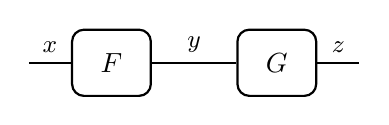
\begin{tikzpicture}[scale=1.05]
\node[process] (f) at (0,0) {$F$};
\node[process] (g) at (2,0) {$G$};
\draw[wire] (-1,0)--(f) node[midway,above,font=\small]{$x$};
\draw[wire] (f)--(g) node[midway,above,font=\small]{$y$};
\draw[wire] (g)--(3,0) node[midway,above,font=\small]{$z$};
\end{tikzpicture}
\vspace{5mm}
{\small Shared wires are eliminated.}
\end{column}
\begin{column}{.48\textwidth}
\hl{Parallel composition}\par
\vspace{3mm}
\centering
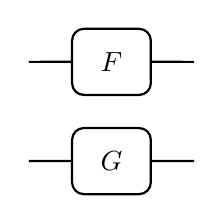
\begin{tikzpicture}[scale=1.05]
\node[process] (f) at (0,.6) {$F$};
\node[process] (g) at (0,-.6) {$G$};
\draw[wire] (-1,.6)--(f);\draw[wire] (f)--(1,.6);
\draw[wire] (-1,-.6)--(g);\draw[wire] (g)--(1,-.6);
\end{tikzpicture}
\vspace{2mm}
{\small Independent blocks add their costs.}
\end{column}
\end{columns}
\tagline{A wire carries a real variable; a box denotes a relation or cost bifunction.}
\end{frame}

% 06 | 50 s
\begin{frame}[t]{Composition already eliminates variables}
\centering
\vspace{2mm}
\begin{tikzpicture}[x=1.3cm,y=1cm]
\node (x) at (0,0) {$x$};
\node[process] (r) at (1.4,0) {$R$};
\node (y) at (2.8,0) {$y$};
\node[process] (s) at (4.2,0) {$S$};
\node (z) at (5.6,0) {$z$};
\draw[wire] (x)--(r);
\draw[wire] (r)--(y);
\draw[wire] (y)--(s);
\draw[wire] (s)--(z);
\node[text=structure,font=\small\bfseries] at (2.8,-.7) {internal};
\end{tikzpicture}
\vspace{5mm}
\[
(S\circ R)(x,z)\iff
\exists y:\;R(x,y)\wedge S(y,z).
\]
\tagline{The external interface retains $x,z$; the shared $y$ disappears.}
\end{frame}

% 07 | 45 s
\begin{frame}[t]{Reformulation can be a change of grouping}
\centering
\begin{tikzpicture}[scale=1.08]
\node[process] (a) at (0,.8) {$A$};
\node[process] (b) at (2.2,.8) {$B$};
\node[process] (c) at (0,-.8) {$C$};
\node[process] (d) at (2.2,-.8) {$D$};
\draw[wire] (-1,.8)--(a);\draw[wire] (a)--(b);\draw[wire] (b)--(3.2,.8);
\draw[wire] (-1,-.8)--(c);\draw[wire] (c)--(d);\draw[wire] (d)--(3.2,-.8);
\draw[structure,dashed,rounded corners] (-.65,-1.3) rectangle (.65,1.3);
\draw[structure,dashed,rounded corners] (1.55,-1.3) rectangle (2.85,1.3);
\end{tikzpicture}
\vspace{2mm}
\[
(B\circ A)\otimes(D\circ C)
=(B\otimes D)\circ(A\otimes C).
\]
\tagline{The wiring is unchanged. Only the way we parse it changes.}
\credit{Monoidal interchange law; dissertation, Introduction. Dashed boxes are grouping guides, not generators.}
\end{frame}

% 08 | 60 s
\begin{frame}[t]{Replace feasibility by cost}
\[
\ind{P}(q)=
\begin{cases}
0,&q\in P,\\
+\infty,&q\notin P.
\end{cases}
\]
\vspace{3mm}
{\small Compose with these indicators and minimize over the shared variable:}
\vspace{2mm}
\tagline{Existential elimination becomes optimal aggregation:
\[
(G\circ F)(x,z)=\inf_y\bigl(F(x,y)+G(y,z)\bigr).
\]
For costs in $\{0,+\infty\}$ this is exactly feasibility of the connection.}
\end{frame}

% 09 | 40 s
\begin{frame}[t]{Quantales explain the shared pattern}
\centering
\vspace{1mm}
\[
(S\circ R)(x,z)=
\bigvee_y R(x,y)\otimes S(y,z).
\]
\vspace{3mm}
\begin{tabular}{lll}
\textbf{Setting}&\textbf{Combine}&\textbf{Aggregate}\\[2mm]
Truth values&$\wedge$&$\exists\ /\ \bigvee$\\[2mm]
Costs&$+$&$\inf$
\end{tabular}
\tagline{Quantale: a complete lattice with a join-preserving monoidal product.}
\end{frame}

\section{The constraint calculus}

% 10 | 40 s
\begin{frame}[t]{Build on the existing graphical languages}
\centering
\vspace{3mm}
\begin{tikzpicture}[x=1cm,y=1cm]
\node[stage] (a) at (0,0) {\textbf{GLA}\\linear};
\node[stage] (b) at (3.3,0) {\textbf{GAA}\\affine};
\node[stage] (c) at (6.6,0) {\textbf{GPA}\\polyhedral};
\node[stage,draw=structure,fill=structure!10] (d) at (9.9,0) {\textbf{GLP}\\LP costs};
\draw[thick] (a)--(b) node[midway,above,font=\small]{$\inlinegen{affine}$};
\draw[thick] (b)--(c) node[midway,above,font=\small]{$\inlinegen{ge}$};
\draw[thick] (c)--(d) node[midway,above,font=\small]{$\inlinegen{linear}$};
\node[font=\small] at (3.1,-1.25) {prior work};
\node[text=structure,font=\small\bfseries] at (9.3,-1.25) {this dissertation};
\end{tikzpicture}
\tagline{Each extension adds expressive power.}
\end{frame}

% 11 | 50 s
\begin{frame}[t]{GPA expresses feasible regions}
\begin{columns}[c,onlytextwidth]
\begin{column}{.38\textwidth}
\centering
\begin{tikzpicture}[scale=1.8]
\pic (g) at (0,0) {ge};
\node[left] at (-.65,0) {$u$};
\node[right] at (.65,0) {$v$};
\end{tikzpicture}
\vspace{4mm}
\[
\sem{\ge}=\{(u,v)\mid u\ge v\}.
\]
\end{column}
\begin{column}{.57\textwidth}
\hl{Matrices + affine constants + order}\par
\vspace{4mm}
\[
P=\{q\mid Mq+r\ge0\}.
\]
\vspace{3mm}
{\small Equalities are pairs of inequalities.}
\end{column}
\end{columns}
\tagline{At this stage every feasible point costs $0$; every infeasible point costs $+\infty$.}
\end{frame}

% 12 | 45 s
\begin{frame}[t]{Projection is the computational primitive}
\centering
\vspace{3mm}
\[
\exists y:\quad y\ge x,\quad z\ge y
\qquad\Longleftrightarrow\qquad z\ge x.
\]
\vspace{4mm}
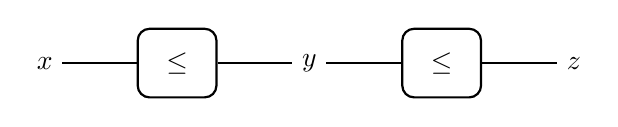
\begin{tikzpicture}[scale=1.2]
\node (x) at (0,0) {$x$};
\node[process] (l) at (1.4,0) {$\le$};
\node (y) at (2.8,0) {$y$};
\node[process] (u) at (4.2,0) {$\le$};
\node (z) at (5.6,0) {$z$};
\draw[wire] (x)--(l);\draw[wire] (l)--(y);
\draw[wire] (y)--(u);\draw[wire] (u)--(z);
\end{tikzpicture}
\tagline{Fourier--Motzkin elimination pairs lower bounds with upper bounds.}
\end{frame}

% 13 | 50 s
\begin{frame}[t]{GPA provides the proof engine}
\hl{Existing result, developed in the draft}\par
\vspace{3mm}
\[
\mathrm{FreeP}_{\GPA}\;\cong\;\PolyRel.
\]
\vspace{3mm}
\begin{columns}[T,onlytextwidth]
\begin{column}{.31\textwidth}
\textbf{Expressivity}\par\vspace{2mm}
{\small Every polyhedral relation has a diagram.}
\end{column}
\begin{column}{.31\textwidth}
\textbf{Soundness}\par\vspace{2mm}
{\small Every allowed rewrite preserves its relation.}
\end{column}
\begin{column}{.31\textwidth}
\textbf{Completeness}\par\vspace{2mm}
{\small Equal relations are equated by the rules.}
\end{column}
\end{columns}
\tagline{Later, LP equality will be transferred to equality of polyhedral relations.}
\end{frame}

\section{The GLP extension}

% 14 | 60 s
\begin{frame}[t]{The new generator assigns linear cost}
\begin{columns}[c,onlytextwidth]
\begin{column}{.34\textwidth}
\centering
\costpic
\vspace{5mm}
\[
\ell:0\longrightarrow1
\]
\end{column}
\begin{column}{.6\textwidth}
\[
\sem{\ell}(\bullet,x)=x.
\]
\vspace{2mm}
{\small The output is a variable, not a chosen optimizer.}\par
\vspace{3mm}
{\small Composition with constraints will optimize over it.}
\end{column}
\end{columns}
\tagline{One scalar cost suffices for arbitrary linear objectives.}
\end{frame}

% 15 | 50 s
\begin{frame}[t]{The semantics: LPs with external interfaces}
{\small A morphism $F:n\to m$ is represented by a value function:}
\[
F(x,y)=
\inf_z\left\{c^\top z\;\middle|\;
Az\ge B\begin{bmatrix}x\\y\end{bmatrix}+r\right\}.
\]
\vspace{3mm}
{\small $x,y$: external variables.\qquad $z$: internal decisions.}\par
\vspace{3mm}
{\small $A,B,c,r$ are fixed; the RHS depends affinely on the interface.}
\tagline{The denotation is a value function, not an optimization algorithm.}
\end{frame}

% 16 | 60 s
\begin{frame}[t]{LP blocks compose into LP blocks}
\[
(G\circ F)(x,w)=\inf_{y,z,z'}
\bigl(c_F^\top z+c_G^\top z'\bigr)
\]
{\centering\small subject to both blocks' linear constraints.\par}
\vspace{2mm}
\[
(F\otimes G)\bigl((x,x'),(y,y')\bigr)
=F(x,y)+G(x',y').
\]
\tagline{Sequential composition eliminates; parallel composition adds costs.}
\end{frame}

% 17 | 60 s
\begin{frame}[t]{Our running LP becomes a diagram}
\centering
\begin{tikzpicture}[scale=1.05]
\pic (l1) at (0,1) {linear};
\pic (l2) at (0,-1) {linear};
\pic[val=2] (s2) at (1.2,-1) {coscalar};
\pic (copy1) at (2.4,1) {copy};
\pic (copy2) at (2.4,-1) {copy};
\pic (bounds1) at (3.6,2.1) {copy};
% Each copied branch checks a bound and terminates at its fixed constant.
\pic (upper1) at (5,2.6) {coge};
\pic (one) at (6.2,2.6) {coaffine};
\pic (lower1) at (5,1.6) {ge};
\pic (zero1) at (6.2,1.6) {cozero};
\pic (lower2) at (5,-1.5) {ge};
\pic (zero2) at (6.2,-1.5) {cozero};
\pic (sum) at (6.8,0) {multiplication};
\pic (demand) at (8.3,0) {ge};
\draw[wire] (l1-out-0)--(copy1-in-0)
  node[midway,above,font=\small]{$x_1$};
\draw[wire] (l2-out-0)--(s2-in-0)
  node[midway,above,font=\small]{$u$};
\draw[wire] (s2-out-0)--(copy2-in-0)
  node[midway,above,font=\small]{$x_2$};
\draw[wire] (copy1-out-0) to[out=0,in=180] (bounds1-in-0);
\draw[wire] (bounds1-out-0)--(upper1-in-0);
\draw[wire] (upper1-out-0)--(one-out-0)
  node[midway,above,font=\small]{$1$};
\draw[wire] (bounds1-out-1)--(lower1-in-0);
\draw[wire] (lower1-out-0)--(zero1-in-0)
  node[midway,above,font=\small]{$0$};
\draw[wire] (copy2-out-1)--(lower2-in-0);
\draw[wire] (lower2-out-0)--(zero2-in-0)
  node[midway,below,font=\small]{$0$};
\draw[wire] (copy1-out-1)--(sum-in-0);
\draw[wire] (copy2-out-0)--(sum-in-1);
\draw[wire] (sum-out-0)--(demand-in-0)
  node[midway,above,font=\small]{$x_1+x_2$};
\draw[wire] (demand-out-0)--(9.4,0) node[right]{$d$};
\node[text=structure,font=\small\bfseries] at (0,1.65) {cost $x_1$};
\node[text=structure,font=\small\bfseries] at (.4,-1.75) {cost $u=2x_2$};
\end{tikzpicture}
\vspace{1mm}
\[
v(d)=\inf\{x_1+2x_2\mid x_1+x_2\ge d,\;0\le x_1\le1,\;x_2\ge0\}.
\]
\end{frame}

% 18 | 50 s
\begin{frame}[t]{Three axioms control the new cost}
\begin{columns}[c,onlytextwidth]
\begin{column}{.58\textwidth}
\centering
\resizebox{\linewidth}{!}{\begin{tabular}{r c c c}
  \diagrow{(linearity)}{
      \pic (g1) at (0.500,1.000) {linear};
      \pic (g2) at (0.500,0.000) {linear};
  }{
      \pic (g1) at (0.500,0.500) {linear};
      \pic (g2) at (1.750,0.500) {comultiplication};
      \draw (g1-out-0) to[out=0,in=180] (g2-in-0);
  }
  \diagrow{(zeroeq)}{
      \pic (g1) at (0.500,0.500) {linear};
      \begin{scope}[shift={(1.250,0.000)}]
      \pic (g2) at (0.500,0.500) {cozero};
      \end{scope}
      \draw (g1-out-0) to[out=0,in=180] (g2-in-0);
  }{
      \node[draw, dotted] {};
  }
  \diagrow{(inf)}{
      \pic (g1) at (0.500,0.500) {linear};
      \begin{scope}[shift={(1.250,0.000)}]
      \pic (g2) at (0.500,0.500) {ge};
      \end{scope}
      \draw (g1-out-0) to[out=0,in=180] (g2-in-0);
  }{
      \pic (g1) at (0.500,0.500) {linear};
  }
\end{tabular}}
\end{column}
\begin{column}{.38\textwidth}
{\small\hl{Their semantic content}}\par
\vspace{4mm}
{\small
Additivity:\quad $\ell(x)+\ell(y)=\ell(x+y)$.\par
\vspace{5mm}
Zero:\quad evaluate the cost at $0$.\par
\vspace{5mm}
Infimum:\quad $\inf_{t\ge x}t=x$.
}
\end{column}
\end{columns}
\tagline{The third axiom is the link between a cost and its epigraph.}
\end{frame}

% 19 | 45 s
\begin{frame}[t]{Expressivity and soundness are direct}
\begin{columns}[T,onlytextwidth]
\begin{column}{.47\textwidth}
\hl{Expressivity}\par
\vspace{4mm}
\begin{enumerate}
\item Encode the linear objective.
\item Encode constraints in GPA.
\item Compose to eliminate decisions.
\end{enumerate}
\end{column}
\begin{column}{.47\textwidth}
\hl{Soundness}\par
\vspace{4mm}
Inherited GPA rules are sound.\par
\vspace{2mm}
Check the three new identities.\par
\vspace{2mm}
Rewrites preserve denotation.
\end{column}
\end{columns}
\tagline{The difficult direction is the converse: can the rules prove \emph{every} value-function equality?}
\end{frame}

\section{Completeness and scope}

% 20 | 45 s
\begin{frame}[t]{Normal form collects the objective}
\centering
\vspace{2mm}
\resizebox{.78\linewidth}{!}{\begin{tikzpicture}
    \pic (g1) at (0.500,1.300) {linear};
    \coordinate (id_in_2) at (0,0.700);
    \coordinate (id_out_3) at (1.000,0.700);
    \draw (id_in_2) -- (id_out_3);
    \pic[val=A] (g4) at (2.000,1.000) {2drelation};
    \draw (g1-out-0) to[out=0,in=180] (g4-in-0);
    \draw (id_out_3) to[out=0,in=180] (g4-in-1);
    \pic (g5) at (3.500,1.000) {ge};
    \draw (g4-out-0) to[out=0,in=180] (g5-in-0);
    \pic[val=B] (g6) at (5.000,1.000) {corelation};
    \draw (g5-out-0) to[out=0,in=180] (g6-in-0);
\end{tikzpicture}
}\par
\vspace{4mm}
\hl{One cost source + a polyhedral constraint block}\par
\vspace{3mm}
{\small Structural induction on generators, sequential composition, and tensor.}
\tagline{A common \emph{shape} for diagrams, not a claim of unique matrices or a unique LP formulation.}
\end{frame}

% 21 | 80 s
\begin{frame}[t]{The epigraph turns cost into geometry}
\begin{columns}[c,onlytextwidth]
\begin{column}{.5\textwidth}
\centering
\epipic
\end{column}
\begin{column}{.46\textwidth}
\[
\epi(v)=\{(d,t)\mid t\ge v(d)\}.
\]
\vspace{3mm}
For our example the shaded region is exactly
\[
t\ge0,\qquad t\ge d,\qquad t\ge2d-1,
\]
a polyhedron, hence a GPA diagram.
\end{column}
\end{columns}
\tagline{Same value function$\Rightarrow$same epigraph: an equality of costs becomes an equality of polyhedra.}
\end{frame}

% 22 | 70 s
\begin{frame}[t]{Epigraph form is a syntactic bridge}
{\small Adding a threshold variable, the epigraph of a value function is a GPA relation $E$, and
$F(q)=\inf\{t\mid(q,t)\in E\}$:}
\vspace{1mm}
\resizebox{.74\linewidth}{!}{\begin{tikzpicture}
  \pic (g1) at (0.500,1.000) {linear};
  \pic (g0) at (1.750,1.000) {ge};
  \draw (g1-out-0) to[out=0,in=180] (g0-in-0);
  \pic (g2) at (3.000,1.000) {comultiplication};
  \draw (g0-out-0) to[out=0,in=180] (g2-in-0);
  \pic[val=A] (g3) at (5.000,1.000) {2drelation};
  \draw (g2-out-0) to[out=0,in=180] (g3-in-0);
  \draw (g2-out-1) to[out=0,in=180] (g3-in-1);
  \pic (g4) at (6.500,1.000) {ge};
  \draw (g3-out-0) to[out=0,in=180] (g4-in-0);
  \pic (g5) at (7.500,1.000) {comultiplication};
  \draw (g4-out-0) to[out=0,in=180] (g5-in-0);
  \pic[val=B] (g6) at (9.000,1.500) {comatrix};
  \draw (g5-out-0) to[out=0,in=180] (g6-in-0);
  \draw (g6-out-0) -- ++(1.000,0);
  \pic (g7) at (8.500,0.500) {antipode};
  \draw (g5-out-1) to[out=0,in=180] (g7-in-0);
  \pic[val=C] (g8) at (10.000,0.500) {comatrix};
  \draw (g7-out-0) to[out=0,in=180] (g8-in-0);
  \draw[dotted] (1.150,-0.050) rectangle (10.750,2.050);
\end{tikzpicture}
}\par
\vspace{1mm}
{\small
\[ \epi([d])=\{(t,y_1,y_2)\mid \exists z\le t:\;Az+a\ge By_1-Cy_2\},\qquad A=[A'\,C]. \]
\[ [d](y_1,y_2)=\inf_{z}\{z\mid Az+a\ge By_1-Cy_2\}. \]
}

\tagline{Crucially, the axioms \emph{rewrite} the diagram into this: one cost source, one GPA block.}
\end{frame}

% 23 | 100 s
\begin{frame}[t]{The completeness argument}
\centering
\begin{tikzpicture}[x=1cm,y=1cm]
\node[proofbox] (v) at (0,1.7) {$\sem{c}=\sem{d}$};
\node[proofbox] (epi) at (5.7,1.7) {$\epi(\sem c)=\epi(\sem d)$};
\node[proofbox] (gpa) at (5.7,.2) {$E_c=E_d$ in GPA};
\node[proofbox] (forms) at (0,-1.3) {$c=\ell;E_c,\quad d=\ell;E_d$};
\node[proofbox,draw=structure,fill=structure!10] (eq) at (5.7,-1.3) {$c=d$ in GLP};
\draw[->,thick] (v)--(epi) node[midway,above,font=\scriptsize]{take epigraphs};
\draw[->,thick] (epi)--(gpa) node[midway,right,font=\scriptsize]{GPA completeness};
\draw[->,thick] (gpa)--(eq) node[midway,right,font=\scriptsize]{attach the same cost};
\draw[->,thick] (forms)--(eq) node[midway,above,font=\scriptsize,align=center]{use epigraph\\rewrites};
\end{tikzpicture}\par
\vspace{2mm}
{\small\hl{Semantic equality yields an equational derivation.}}
\end{frame}

% 24 | 60 s
\begin{frame}[t]{Simplify the example: collect cost, then eliminate}
\centering
{\small\hl{1. Linearity collects the two cost sources.}}\par
\begin{tikzpicture}[scale=.8]
\pic (a) at (0,.5) {linear};
\pic (b) at (0,-.5) {linear};
\draw[wire] (a-out-0)--(1.2,.5) node[right] {$x_1$};
\draw[wire] (b-out-0)--(1.2,-.5) node[right] {$u=2x_2$};
\node at (3,0) {$=$};
\pic (cost) at (4,0) {linear};
\pic (split) at (5.3,0) {comultiplication};
\draw[wire] (cost-out-0)--(split-in-0) node[midway,above] {$c$};
\draw[wire] (split-out-0)--(6.5,.5) node[right] {$x_1$};
\draw[wire] (split-out-1)--(6.5,-.5) node[right] {$u=2x_2$};
\node[font=\small] at (5.5,-1.05) {$c=x_1+2x_2$};
\end{tikzpicture}\par
{\small\hl{2. The (inf) rule introduces $t\ge c$; GPA projects the decisions.}}
{\small
\[
 s=x_1+x_2,\quad c=2s-x_1:
 \qquad \max\{0,2s-t\}\le x_1\le\min\{1,s\}.
\]
\[
 \underset{\text{GPA / Fourier--Motzkin: eliminate }x_1}{\Longleftrightarrow}
 s\ge0,\quad t\ge s,\quad t\ge2s-1,\quad s\ge d.
\]
\[
 \underset{\text{GPA / Fourier--Motzkin: eliminate }s}{\Longleftrightarrow}
 \boxed{t\ge0,\qquad t\ge d,\qquad t\ge2d-1.}
\]
}
{\footnotesize Each projection is an inherited GPA rewrite; redundant bounds are removed.}
\end{frame}

% 25 | 60 s
\begin{frame}[t]{The simplified diagram has no source decisions}
\centering
\resizebox{!}{4cm}{%
\begin{tikzpicture}
\pic (cost) at (0,0) {linear};
\pic (split) at (1.3,0) {copy};
\pic (split2) at (2.5,-.5) {copy};
\pic (nonnegative) at (3,1.5) {ge};
\pic (zero) at (4.3,1.5) {cozero};
\pic (first) at (4,0) {ge};
\pic (one) at (2.5,-2) {affine};
\pic (add) at (4,-1.5) {multiplication};
\pic[val={\frac12}] (half) at (5.3,-1.5) {scalar};
\pic (second) at (6.5,-1.5) {ge};
\pic (merge) at (8,-.5) {cocopy};
\draw[wire] (cost-out-0)--(split-in-0) node[midway,above] {$t$};
\draw[wire] (split-out-0) to[out=0,in=180] (nonnegative-in-0);
\draw[wire] (nonnegative-out-0)--(zero-in-0) node[midway,above] {$0$};
\draw[wire] (split-out-1)--(split2-in-0);
\draw[wire] (split2-out-0)--(first-in-0);
\draw[wire] (first-out-0)--(merge-in-0) node[midway,above] {$d$};
\draw[wire] (split2-out-1)--(add-in-0);
\draw[wire] (one-out-0)--(add-in-1) node[midway,below] {$1$};
\draw[wire] (add-out-0)--(half-in-0) node[midway,above] {$t+1$};
\draw[wire] (half-out-0)--(second-in-0);
\draw[wire] (second-out-0) to[out=0,in=180] (merge-in-1);
\draw[wire] (merge-out-0)--(9,-.5) node[right] {$d$};
\node[font=\small,anchor=west] at (4.8,1.5) {$t\ge0$};
\node[font=\small,anchor=north] at (6,-2.15) {$(t+1)/2\ge d$};
\end{tikzpicture}%
}\par
\vspace{1mm}
\[
 v(d)=\inf\{t\mid t\ge0,\ t\ge d,\ t\ge2d-1\}
     =\max\{0,d,2d-1\}.
\]
{\small\hl{Linearity + (inf) + GPA: two decisions become one cost wire.}}
\end{frame}

% 26 | 60 s
\begin{frame}[t]{Result, scope, and remaining work}
\[
\mathrm{FreeP}_{\GLP}\;\cong\;\LPRel
\]
\begin{columns}[T,onlytextwidth]
\begin{column}{.48\textwidth}
\hl{Presented in this work}\par
\vspace{3mm}
{\small RHS-parametric value functions.\par
\vspace{1mm}
One generator; three axioms.\par
\vspace{1mm}
Normal form and completeness.}
\end{column}
\begin{column}{.48\textwidth}
\end{column}
\end{columns}
\end{frame}

% 27 | 35 s
\begin{frame}[t]{Optimization becomes part of the syntax}
\hl{Composition eliminates internal decisions.}\par
\vspace{5mm}
\hl{Equations certify equality of value functions.}\par
\vspace{5mm}
\large{Thank you. Questions?}
\end{frame}

\end{document}
